\chapter{Introduction to the problem}\label{cap:Introduction}
In this report, we present an algorithm for the so-called \textit{SLAM} problem. This is one of the most challenging problems in the robotics research area, and its acronym stands for Simultaneous Localization and Mapping. Its aim is to reconstruct the trajectory and the map of an environment a mobile entity moves into, given some data.
Data could be robot poses, camera images associated to these poses, sonar acquisitions and many more.
Needless to say, these data are usually affected by noise, meaning that solving SLAM problems usually involves a certain level of uncertainties.

\section{Graph model}
A quite suitable way to represent our knowledge about the world is using a graph.
In such a graph (see figure \ref{fig:graph}):
\begin{itemize}
  \item Nodes are either robot poses or landmarks.
  \item Edges are constraints between nodes.
\end{itemize}
\begin{figure}[htbp]
  \centering
    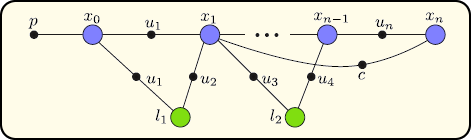
\includegraphics[width=0.5\textwidth]{images/graph.png}
  \caption{World representation graph. Blue nodes are poses, green ones are landmarks.}
  \label{fig:graph}
\end{figure}
This way, you can imagine the graph as a lot of blocks (the nodes), with springs (the edges) that ``pull and push'' these blocks.
If there were no errors, these springs wouldn't conflict each other. The presence of errors leads to the needing of finding a compromise state.
The solution that minimizes the overall ``conflict force'' is the one that we choose as guess about the world. The search for such a state is called optimization.

\section{Our case: bearing only sensor}
%% We want to generate a 2D map of the environment and to adjust the trajectory of the robot.

In order to infer something about the world, the first step is to gather data, and to associate them in a proper way.

The algorithm for data association that we developed assumes that the robot is equipped with a bearing sensor. A bearing sensor is a sensor that detects an interesting point and returns, as information, the ``direction'' (actually an angle) where it is situated with respect to the robot.
This sensor is of course an abstraction, but can be assimilated to real sensors in certain conditions.\footnote{For instance an omnidirectional camera used for detecting coloured landmarks}

\begin{figure}[htbp]
  \centering
    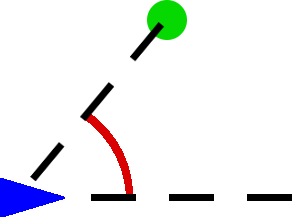
\includegraphics[width=0.3\textwidth]{images/bearing_sensor.png}
  \caption{The sensor detects the red angle.}
  \label{fig:bearing_sensor}
\end{figure}

Since the only information we get about the landmarks is an angle with respect to a robot pose, introducing landmarks in the graph is not as trivial as it would be with other sensor types. This part will be examined in chapter \ref{cap:Algorithm}.

Even after the association has been done, the graph needs a dedicated kind of edge that links a robot pose to a landmark via the direction in which the landmark is seen from the robot pose. This actually constrains the detected angle and the angle computed backprojecting the estimated position of the landmark.
